\begin{task}{62}
Вершины графа ниже занумерованы по возрастанию слева направо (номера вершин обозначены на рисунке), сверху вниз. Запишите, как этот граф будет раскрашен жадным алгоритмом. Использует ли при этом алгоритм наименьшее возможное для данного графа число цветов? Если да, то докажите, что в меньшее число цветов граф раскрасить нельзя. Если нет, то приведите новую нумерацию вершин графа, при которой алгоритм построит оптимальную раскраску.

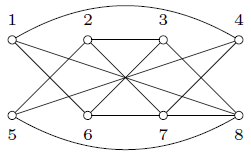
\includegraphics[width = 200pt]{img/id62.png}
\end{task}
\begin{solution}
Граф, раскрашенный жадным алгоритмом, выглядит следующим образом:

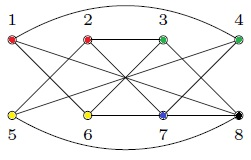
\includegraphics[width = 200pt]{img/id62_greedy.jpg}

Жадный алгоритм использует 5 цветов. Этот результат можно улучшить, перенумеровав вершины:

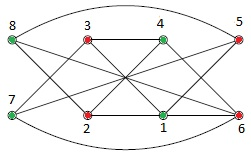
\includegraphics[width = 200pt]{img/id62_optimal.jpg}

С новой нумерацией жадный алгоритм использует всего 2 цвета.
\end{solution}